\section{Question 5}

\subsection{Question}
\verbatiminput{q5/q5.txt}

\subsection{Answer}

To answer this question, {\tt matrix.py} was modified to add the capability to calculate {\it Term Frequency Inverse Document Frequency (TF/IDF)}. The added functions for computing TF/IDF are found in Listing \ref{listing:tfidf}. These functions use the master word count dictionary ({\tt wordcounts}) and each blog's individual word count ({\tt wc}) for each of the words in the {\tt wordlist} from Question 1/2 to compute the TF/IDF value for each word in the word list. 

\lstinputlisting[language=Python, caption={use of tfidf function},label=listing:tfidfmain,linerange={116-117},firstnumber=116]{matrix.py}

\lstinputlisting[language=Python, caption={writing the data}, label=listing:matrix:writedata, linerange={79-93}, firstnumber=79]{matrix.py}

\lstinputlisting[language=Python, caption={tf idf functions},label=listing:tfidf,linerange={40-48},firstnumber=40]{matrix.py}

The same clustering was applied to the TF/IDF result matrix as was done in Question 2 and both images are displayed in Figures \ref{fig:plain} and \ref{fig:tfidf}.

There are a many pairs that were found to be similar in both clusterings. For example, in both dendrograms, the {\it Web Science and Digitial Libraries Research Group} blog is most similar to the {\it ...: zero pride and even less shame} blog, the {\it DJ DHANIEL FAN AND PRODUCER} and {\it The Baron Boombox}, among a few others. In spite of this, the larger groupings do not appear very similar between the two clustings.

When examining the clusters on a larger scale, it seems that the TF/IDF dendrogram clustered blogs are subjectively more alike better than the raw count version did. Looking toward the bottom of the TF/IDF clustering image, one will notice a grouping of blogs that seem closely related to music: {\it F-Measure: Less Than timely Music Reviews and Commentary.}, {\it Urban Anatomy's Columbian Jungle (That Dope!)} which seems to be a melding of fashion and music commentary, {\it Ezhevika Fields} a blog where info and preview samples of ``lost album samples of the past'' can be found, whereas these blogs are not all grouped together in the raw count version. It seems that using TF/IDF as a basis for document comparison gives much more context than a raw term count (which doesn't take into consideration the rest of the document in which each word resides).

There is another cluster in the TF/IDF driven image that seems to contain family related blogs, with blogs like {\it Am I a funny girl?: I think I have my moments}, {\it The Frixen Family}, {\it When Two Hearts Become One: A wife, a mom, a daughter, a sibling.} and {\it The Clarks in Austin} all being related to a particular family and their everyday lives. Some of these blogs are close to each other in the raw count version, but they are not separated into their own distinct groups.

When looking at the overall structure of each dendrogram, it becomes apparent that there are more individual clusters grouped together in the TF/IDF version than are present in the raw count image, where there seems to be few small clusters and one mega-cluster in the center. This suggests that the TF/IDF algorithm is better at defining discrete subgroups within a larger context than a simple raw count driven dendrogram will produce.

\begin{figure}[h!]
\centering
\fbox{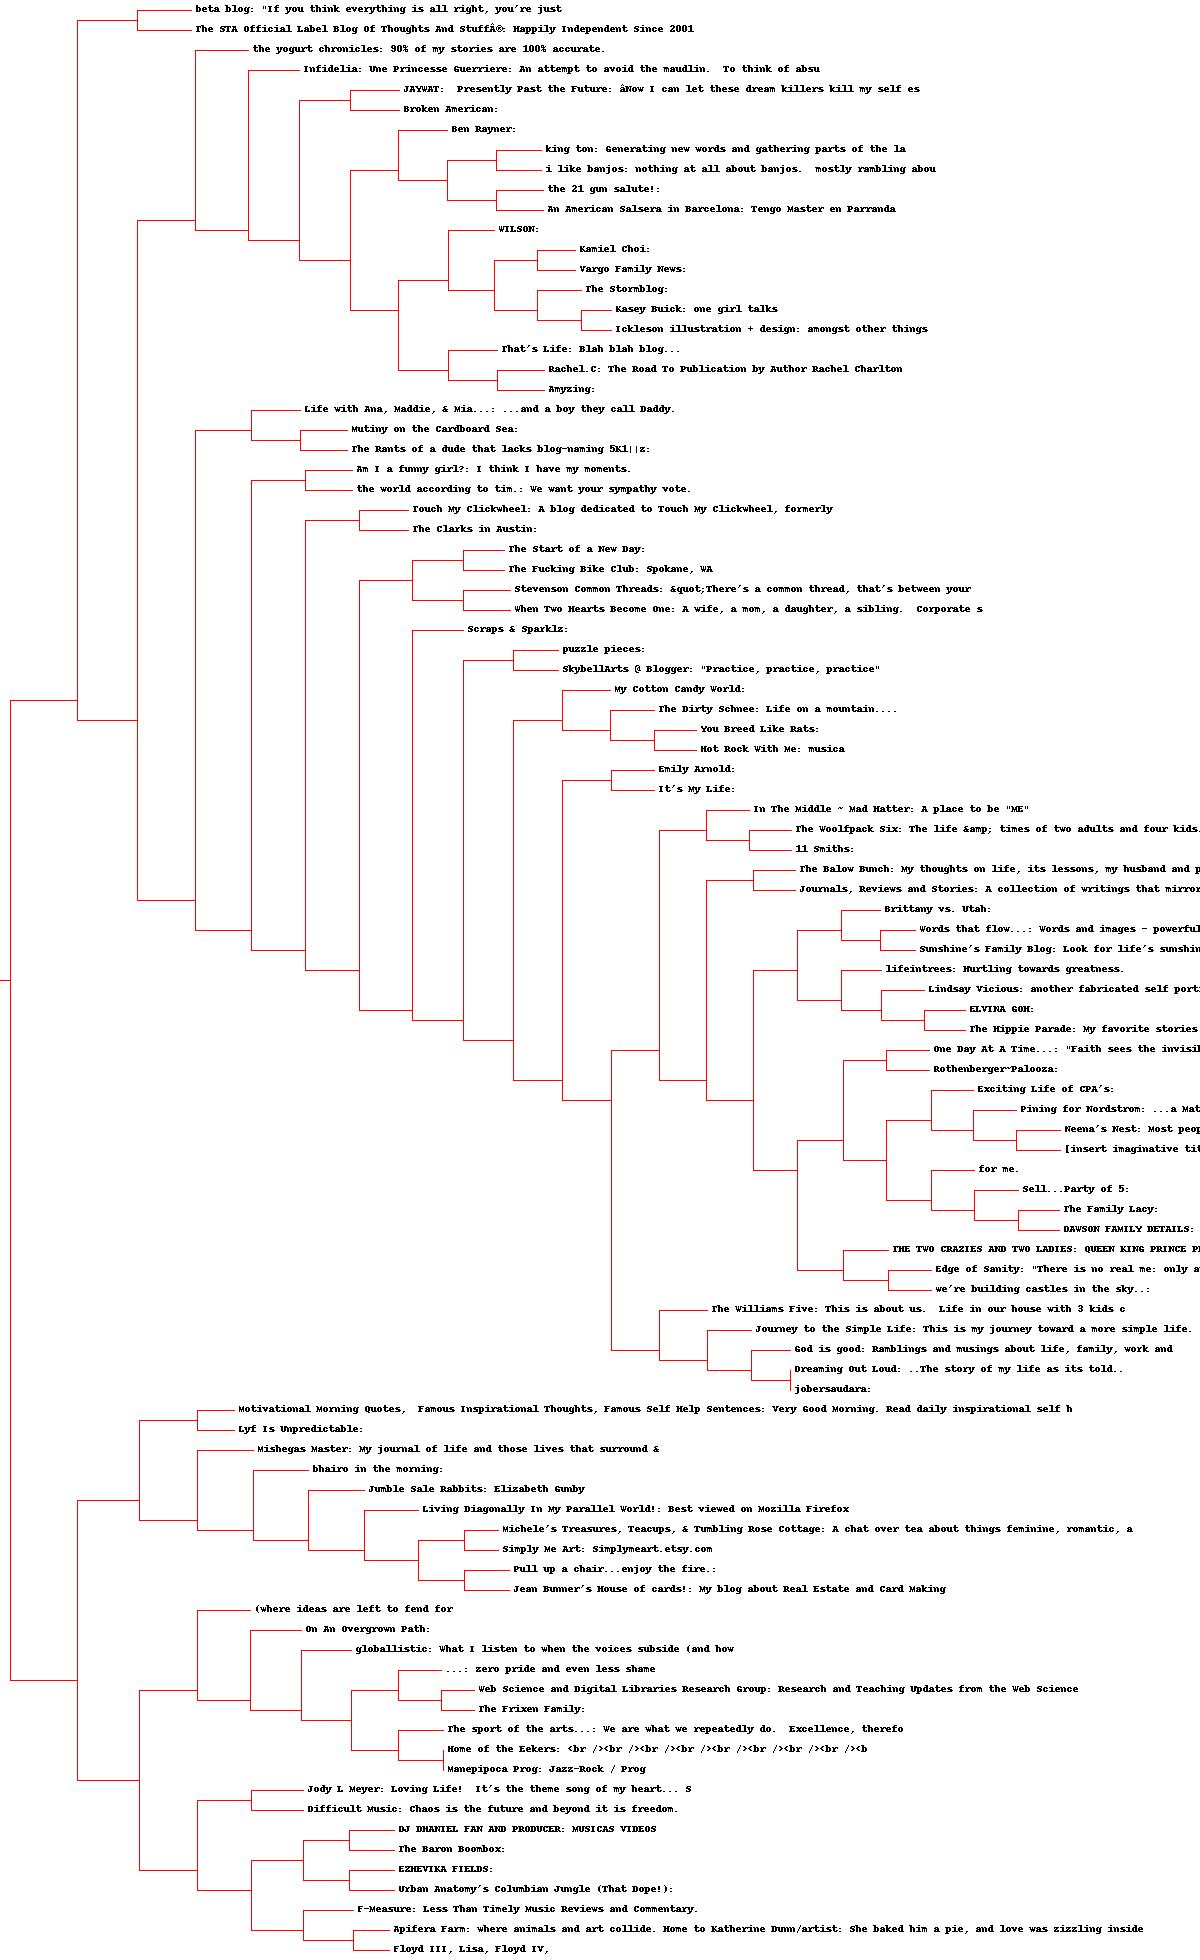
\includegraphics[scale=0.3]{q2/blogclust.jpg}}
\caption{plain count dendrogram}
\label{fig:plain}
\end{figure}

\begin{figure}[h!]
\centering
\fbox{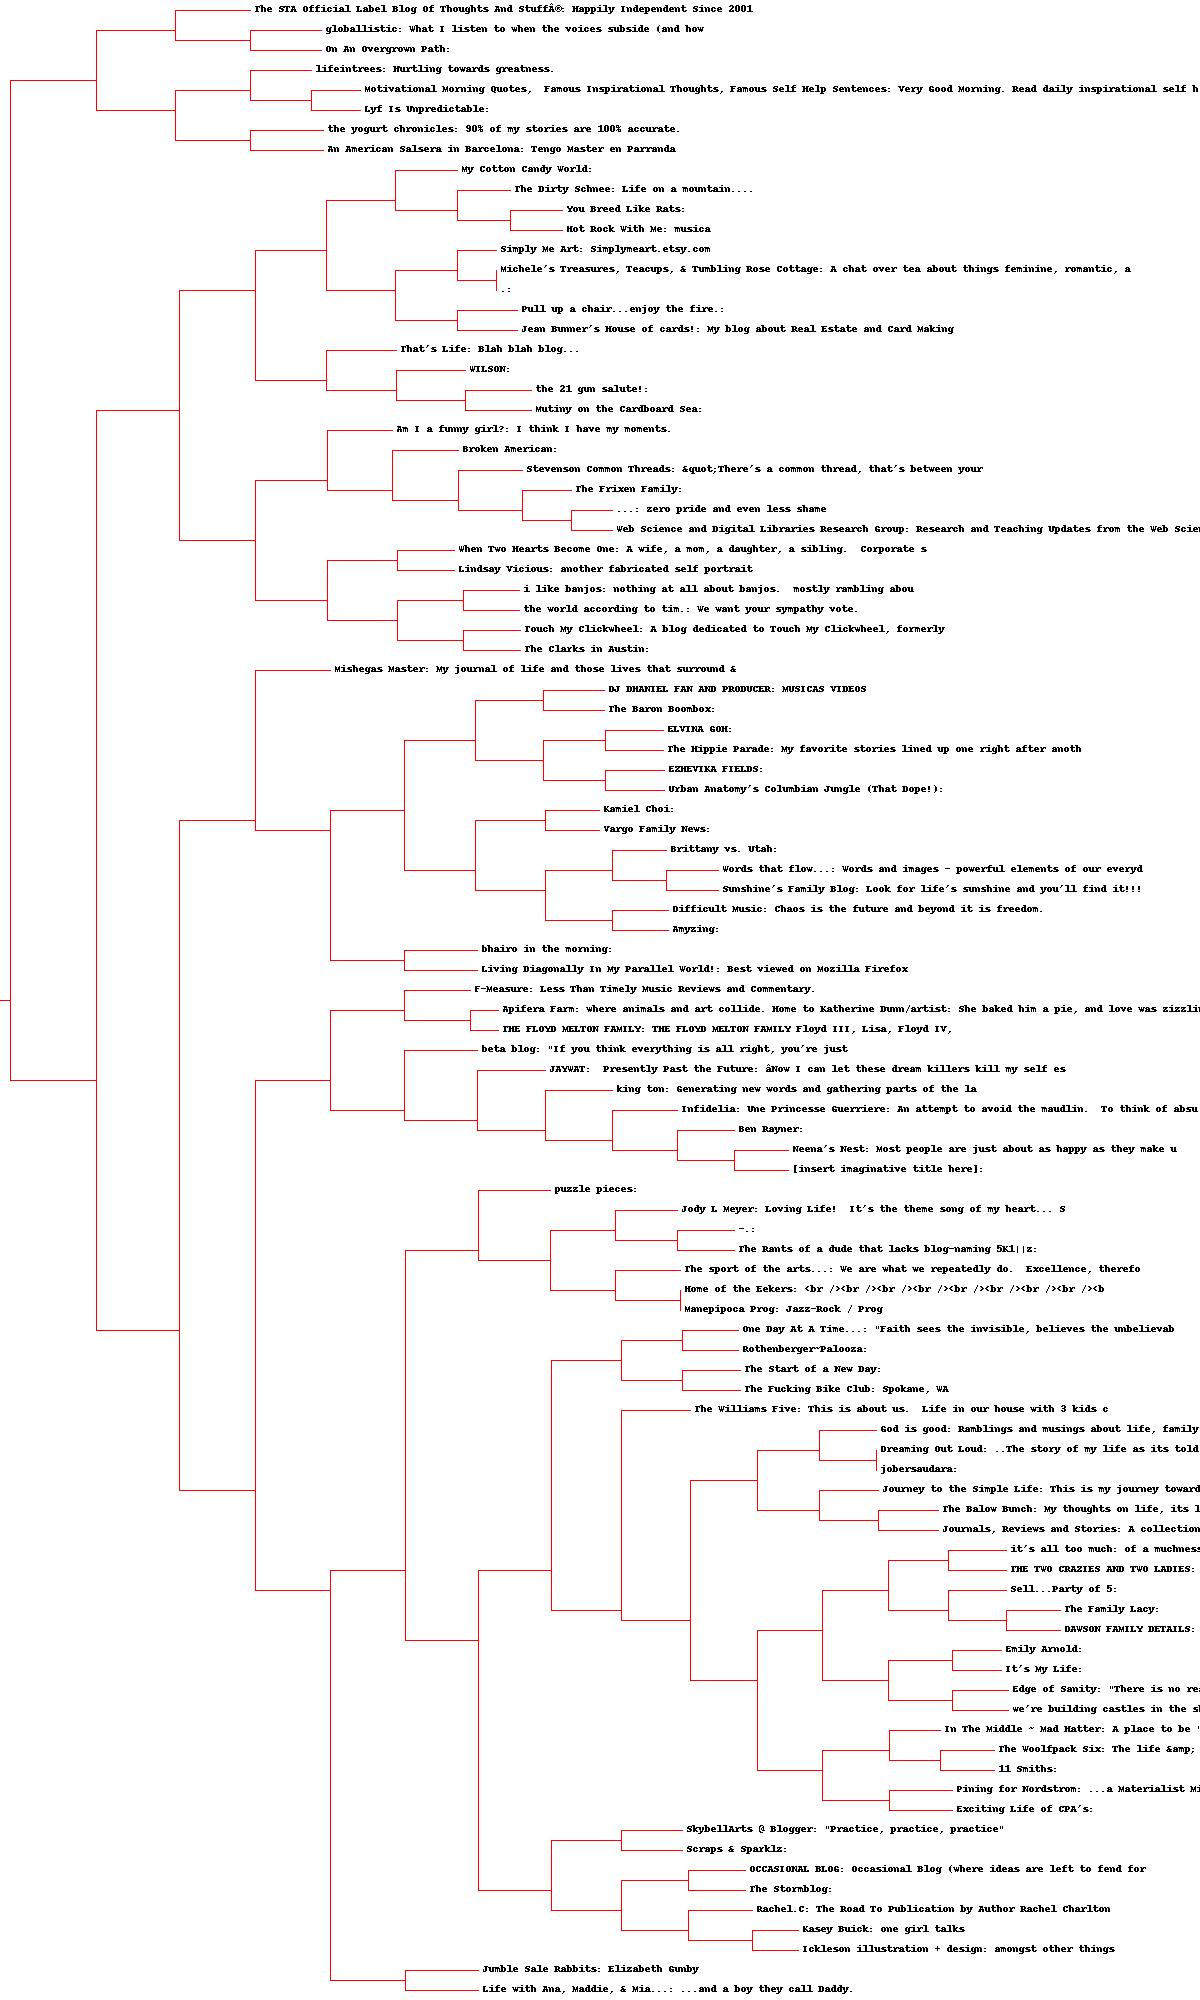
\includegraphics[scale=0.3]{q5/blogclust.jpg}}
\caption{TF/IDF driven dendrogram}
\label{fig:tfidf}
\end{figure}